% D7065E final report, Group 2. Compile with pdflatex; images live next to this file.
\documentclass[11pt,a4paper]{article}
\usepackage[margin=25mm]{geometry}
\usepackage[T1]{fontenc}
\usepackage{lmodern,tabularx,longtable,booktabs,xcolor,amsmath,graphicx,fancyhdr,pgfplots,tikz}
\usepackage{float}
\usepackage{array}
\usepackage{needspace}
% Red placeholders: every \fillin{...} must be replaced before submission.
\newcommand{\fillin}[1]{\textcolor{red}{[#1]}}
\usepackage[hidelinks]{hyperref}
% Images live next to this file (report/). Upload the whole folder to Overleaf.
\graphicspath{{./}}
\pgfplotsset{compat=1.18}
\usetikzlibrary{arrows.meta,positioning,fit,backgrounds,shapes.geometric,babel}
\definecolor{serviceblue}{HTML}{DBEAFE}
\definecolor{devicegreen}{HTML}{DCFCE7}
\definecolor{infrapurple}{HTML}{EDE9FE}
% Shared diagram styles: native centimetres; never scale a TikZ picture.
\newdimen\diagramwidth
\newcommand{\checkdiagramwidth}{%
  \pgfextractx{\diagramwidth}{\pgfpointdiff
    {\pgfpointanchor{current bounding box}{west}}
    {\pgfpointanchor{current bounding box}{east}}}%
  \typeout{REPORT-DIAGRAM-WIDTH: \the\diagramwidth}%
  \ifdim\diagramwidth>15.5cm
    \PackageError{report-diagrams}{Diagram exceeds 15.5 cm}
      {Reduce spacing or split the diagram. Do not scale it.}%
  \fi
  \ifdim\diagramwidth>\linewidth
    \PackageError{report-diagrams}{Diagram exceeds linewidth}
      {Reduce spacing or split the diagram. Do not scale it.}%
  \fi}
\tikzset{
  every picture/.style={font=\small,execute at end picture=\checkdiagramwidth},
  msg/.style={-{Latex[length=2.5mm]}, thick},
  ret/.style={-{Latex[length=2.5mm]}, thick, dashed},
  act/.style={draw, thick, fill=blue!8, minimum width=2.1cm, minimum height=0.7cm, font=\small\bfseries, align=center},
  note/.style={draw, fill=yellow!15, font=\footnotesize, align=left, inner sep=3pt},
  phase/.style={font=\footnotesize\bfseries, text=darkgray, fill=white, inner sep=1pt, anchor=west},
  lbl/.style={above, font=\footnotesize, fill=white, inner sep=1pt, align=center},
  service/.style={act,fill=serviceblue},
  infrastructure/.style={act,fill=infrapurple},
  device/.style={act,fill=devicegreen},
  external/.style={act,fill=gray!12},
  frame/.style={draw=gray,dashed,rounded corners=2pt,inner sep=4pt},
  check/.style={diamond,draw,thick,fill=blue!8,aspect=2,align=center,font=\small,inner sep=2pt},
  process/.style={draw,thick,fill=serviceblue,align=center,font=\small,inner sep=5pt}
}
\newcommand{\diagramphase}[3]{%
  \draw[gray!55,thin] (0,#1) -- (#2,#1);
  \node[phase] at (0.05,#1) {#3};}
\newcommand{\diagramlegend}{\par\smallskip{\footnotesize
  Blue: project service; purple: messaging/storage/dashboard infrastructure;
  green: device adapter; grey: course/external service.\par}}
\pagestyle{fancy}\fancyhf{}
\fancyhead[L]{CO2 ventilation -- Group 2}\fancyhead[R]{D7065E -- Architecture Document}
\fancyfoot[C]{\thepage}\setlength{\headheight}{14pt}
\setlength{\emergencystretch}{3em}
\title{CO\textsubscript{2}-driven ventilation with thermal trade-off\\\large D7065E, Architecture Document}
\author{Group 2: Tobias Hanke \& Evangelos Vasilaras}
\date{12 October 2026}
\begin{document}
{\let\newpage\relax\maketitle}
\tableofcontents
\newpage
\section{Summary}
The system autonomously regulates ventilation and heating in five simulated rooms on level 0 of the A-house. Occupants generate CO\textsubscript{2}; fresh air removes it but also creates a heating demand. Separate sensor, controller and actuator processes close this feedback loop through MQTT and BuildSim. A reactive controller provides threshold-based responses, while an advisory planner uses lecture bookings to anticipate occupancy over 30 simulated minutes. The planner reads observed history, rather than physical ground truth, and its suggestions can raise the reactive ventilation request. JSONL/Parquet storage supports history, audit and evaluation; BuildSim overlays and Grafana expose the resulting conditions and decisions. The guiding principle is that the reactive loop works on its own, while forecasting may only add ventilation or preheating, never remove it.

On one simulated weekday, timetable planning removed the lecture-room CO\textsubscript{2} exceedances (122 to 0 sim-min) at about 9\% more heating energy than reactive control alone. Against a fixed schedule the system used 37\% less energy, but the schedule also kept the lecture rooms below 1000 ppm and gave higher comfort; the 90\% comfort target (FR-02) is not met (Section~\ref{sec:results}).

\noindent\begin{tabularx}{\linewidth}{lX}\toprule Field & Value\\\midrule
Project & CO\textsubscript{2}-driven ventilation with thermal trade-off\\
Team & Group 2: Tobias Hanke; Evangelos Vasilaras\\
Scope & A109, A117, A110, A323 and A113C on level 0\\
Repository & \url{https://github.com/TobiMacaronisGit/d7065e-group2}\\
Version & Branch \texttt{main} at submission, 12 October 2026\\\bottomrule
\end{tabularx}

\paragraph{Changes since the proposal.}
The proposed four-to-six-room demonstration now uses five named rooms with explicit lecture, fika and office roles. Reactive control and planning are separate processes, allowing the reactive path to continue when history or planning is unavailable. MQTT distributes observations and commands; JSONL, Parquet and DuckDB provide inspectable history without a separate database server.

A fitted linear occupancy model lost to persistence on a held-out date and was not deployed; lecture bookings provide the primary forecast instead. In early runs a full lecture room stayed at about 1300--1400 ppm even at the highest ventilation level: at 1.3 air changes per hour (ACH) per level, that level supplied only about 6 l/s per person, below the roughly 7 l/s per person that Swedish public-health guidance recommends for seated activity in schools (\href{https://www.fohm.se/contentassets/641784832543443ea4eebe9b300c244e/fohmfs-2014-18.pdf}{FoHMFS 2014:18}). Ventilation per level was therefore raised to 3.6 ACH, so level 2 now supplies more than 10 l/s per person. Early runs also showed zero occupied comfort, so tempered supply air with heat recovery and stronger radiators were added.

\section{Use case and building context}
\paragraph{Purpose and responsibilities.}
The use case is occupied-room air quality with a thermal and energy trade-off in the A-house. A lecture causes a rapid increase in people and CO\textsubscript{2}; ventilation dilutes the concentration, while heating must replace envelope and fresh-air losses. Advance knowledge of a booking can therefore justify ventilation and preheating before people arrive. A building manager observes the autonomous decisions, their reasons and room conditions. Occupants influence demand through presence; there is no implemented manual-override workflow or approval step for each command.

BuildSim is provided infrastructure holding room geometry, equipment, occupancy, sensor values and reached actuator states, with a browser-based 3D view. The course occupancy simulator supplies people, lecture bookings and the simulated clock. The project supplies room physics, simulated devices, control, planning, history and the dashboard. BuildSim only holds shared state; it neither simulates physics nor makes decisions.

\needspace{9\baselineskip}
\paragraph{Rooms and scenario.}\mbox{}\par
\noindent\begin{tabularx}{\linewidth}{llrrX}\toprule Room & Role & Area (m$^2$) & Volume (m$^3$) & Demand pattern\\\midrule
A109 & Lecture & 188 & 564 & Scheduled class arrivals\\
A117 & Lecture & 214 & 642 & Several scheduled classes\\
A110 & Fika & 124 & 372 & Unscheduled shared-space occupancy\\
A323 & Office & 17 & 51 & Small-room occupancy\\
A113C & Office & 16 & 48 & Small-room occupancy\\\bottomrule\end{tabularx}
All rooms use a 3-m model height and level-qualified identities such as \protect\path{level0/A109}. Each room has one CO\textsubscript{2} sensor, one temperature sensor, one ventilation actuator and one heating actuator (20 device containers); occupancy comes from one shared counter. The one-shot seed process overrides occupancy-simulator roles so lectures occur in the selected rooms. This concentrates useful activity in the demonstration area and narrows how representative its results are.

The recorded evaluation uses simulated Wednesday 21 October 2026, 07:30--18:00, at 60 simulated seconds per wall second. A109 is booked 08:15--10:00 for 101 students; A117 has bookings at 10:15--12:00, 13:15--15:00 and 15:15--17:00 for 97, 115 and 102 students. The simulator models early student and lecturer arrival. A110 and the offices have no lecture bookings, so their planner normally uses persistence.

\section{Requirements}
Times are given either in simulated time (sim-min) or in real time measured by the wall clock (s wall); at the clock factor of 60 used here, one wall second corresponds to one simulated minute. Table~\ref{tab:req} traces the acceptance criteria to the architecture and verification plan.
{\small\begin{longtable}{>{\raggedright\arraybackslash}p{15mm}>{\raggedright\arraybackslash}p{13mm}>{\raggedright\arraybackslash}p{77mm}>{\raggedright\arraybackslash}p{37mm}}
\caption{Requirements and traceability. Type: F functional, NF non-functional, R regulatory, S safety. U1 is the unit-test suite (Section~\ref{sec:tests}).}\label{tab:req}\\
\toprule ID & Type, prio & Acceptance criterion & Design / verification\\\midrule\endfirsthead
\toprule ID & Type, prio & Acceptance criterion & Design / verification\\\midrule\endhead
FR-01 & F, Must & Occupied-room CO\textsubscript{2} returns below 1000 ppm within 10 sim-min after exceeding it. & Reactive rules; U1, S1.\\
FR-02 & F, Must & At least 90\% of occupied sim-min are within 20--24 $^\circ$C over a weekday. & Setpoints, physics; S1.\\
FR-03 & F, Must & Within 15 sim-min of a room emptying, ventilation drops to its minimum and the heating setpoint to the 17 $^\circ$C setback for empty rooms. & Setback rules; U1, S1.\\
FR-04 & F, Should & Forecasting reduces occupied CO\textsubscript{2} exceedance minutes by at least 50\% relative to reactive-only on the same day/seed. & Planner; U1, E3, E5.\\
FR-05 & F, Should & Decisions contain reasons and inputs and can be retrieved from history. & Decision schema, pipeline; U1, audit.\\
NFR-01 & NF, Must & Median per-room decision interval is at most 60 s wall under five-room load. & Five-second control loop; E4.\\
NFR-02 & NF, Must & After a process crash/restart, correct commands resume within 60 s wall without unsafe intervening commands. & Process isolation, reconnect/restart; F3/F4.\\
NFR-03 & NF, Should & No actuator target changes more than once per 5 sim-min, except SAFETY. & Hysteresis/dwell; U1, E2.\\
NFR-04 & NF, Should & Weekday modelled heating energy is no greater than a fixed-schedule baseline. & Occupancy setback; E1.\\
NFR-05 & NF, Must & Frozen CO\textsubscript{2} is detected within 10 sim-min; control continues from occupancy in DEGRADED mode. & Quality classifier; U1, F1/F2.\\
NFR-06 & NF, Should & Following a BuildSim restart, devices re-register and readings resume within 60 s wall without reseeding. & Device self-registration; F5.\\
NFR-07 & NF, Should & A 60-s-wall pipeline outage loses no readings. & QoS 1 and persistent consumer session; F4.\\
REG-01 & R, Must & Every ventilation command is at least the configured minimum, in every mode. & Final clamp; rule review.\\
SAF-01 & S, Must & Reject commands with an incorrect issuer, out-of-range target or wall age over 120 s. & Actuator validation; U1, F6.\\\bottomrule
\end{longtable}}

\section{Architecture}
\subsection{Context diagram (C4 Level 1)}
Figure~\ref{fig:context} shows the system as one box. Occupants affect it only through their presence, which occupancysim simulates; occupancysim also provides the simulated clock and the lecture bookings. BuildSim holds the shared building state and shows it in a 3D view in the browser. The building manager follows room conditions and decisions there and in Grafana, but does not intervene.
\begin{figure}[H]\centering
\begin{tikzpicture}
\node[external,text width=3cm] (people) at (1.8,0) {Occupants};
\node[external,text width=3cm] (manager) at (12.6,0) {Building manager};
\node[external,text width=3cm,minimum height=1.8cm] (occ) at (1.8,-3.2)
 {occupancysim\\\normalfont People, bookings, clock};
\node[service,text width=4cm,minimum height=2.2cm] (sys) at (7.2,-3.2)
 {Ventilation and\\climate control\\\normalfont Five rooms on level 0\\Physics, devices, control,\\planning and history};
\node[external,text width=3cm,minimum height=2.2cm] (bs) at (12.6,-3.2)
 {BuildSim\\\normalfont Shared occupancy,\\values, reached states;\\browser 3D view};
\draw[msg] (people.south) -- node[lbl,xshift=-0.8cm]{presence} (occ.north);
\draw[ret] (occ.north east) -- (3.45,-1.6) -- node[lbl]{clock + bookings\\{}[REST]} (5.03,-1.6) -- (sys.north west);
\draw[ret] (bs.west) -- node[lbl]{room inputs\\{}[REST]} (sys.east);
\draw[msg] (sys.south east) -- (8,-4.9) -- node[lbl]{values / states / view [REST]} (11.8,-4.9) -- (bs.south west);
\draw[msg] (occ.south) -- (1.8,-5.65) -- node[lbl]{occupancy + entities [REST]} (13.4,-5.65) -- (bs.south east);
\draw[msg] (sys.north) -- (7.2,-1.1) -- node[lbl]{history / decisions [HTTP]} (12.6,-1.1) -- (manager.south);
\draw[ret] (bs.east) -- (14.55,-3.2) -- (14.55,0.9) -- node[lbl]{3D view [WebSocket]} (12.6,0.9) -- (manager.north);
\end{tikzpicture}
\par\smallskip{\footnotesize Blue: our system; grey: external actors and provided services.\par}
\caption{System context. Solid arrows show messages/writes; dashed arrows show read or browser responses. Room inputs are occupancy and reached actuator states. Writes include sensor values, reached states, room layers and alerts. Protocols are given in brackets; the presence edge is simulated by occupancysim, not a network call.}\label{fig:context}
\end{figure}

\subsection{Container diagram (C4 Level 2)}
The container diagram separates observation, decisions and actuation into processes. It is split into two figures: Figure~\ref{fig:containers} shows the live feedback loop, Figure~\ref{fig:containers-support} planning, history, dashboard and setup. Broker, BuildSim and occupancysim appear in both. Grouping ten sensors or actuators in a box does not imply a shared process.
\begin{figure}[H]\centering
\begin{tikzpicture}
\node[service,text width=3cm] (phy) at (1.95,0) {physics\\\normalfont Python; 8090\\CO$_2$, heat, energy};
\node[external,text width=3cm] (bs) at (7.35,0) {BuildSim\\\normalfont Go; 9090\\Occupancy, states};
\node[external,text width=3cm] (occ) at (12.75,0) {occupancysim\\\normalfont Go; 8081\\People, clock,\\bookings};
\node[device,text width=3cm] (sen) at (1.95,-3.5) {sensor-* $\times10$\\\normalfont Python; 2 s wall\\CO$_2$/temperature};
\node[device,text width=3cm] (cnt) at (12.75,-3.5) {occupancy\_\\counter\\\normalfont Python; 2 s wall\\Shared container};
\node[infrastructure,text width=3cm] (mq) at (7.35,-6.5) {broker\\\normalfont Mosquitto\\MQTT 1883; QoS 1\\Retained targets};
\node[device,text width=3cm] (act) at (1.95,-9.4) {actuator-* $\times10$\\\normalfont Python; vent / heat\\Validate and move};
\node[service,text width=3cm] (ctl) at (12.75,-9.4) {control\\\normalfont Python; 8091\\Every 5 s wall};
\draw[ret] (bs.west) -- node[lbl]{room inputs\\{}[REST]} (phy.east);
\draw[msg] (occ.west) -- node[lbl]{occupancy\\{}[REST]} (bs.east);
\draw[ret] (phy.south) -- node[lbl,xshift=1cm]{room truth [REST]} (sen.north);
\draw[ret] (bs.south east) -- node[lbl]{persons [REST]} (cnt.north west);
\draw[msg] (sen.east) -- node[lbl]{observations\\{}[MQTT]} (6.75,-3.5) -- (mq.north west);
\draw[msg] (cnt.west) -- node[lbl]{head counts\\{}[MQTT]} (7.95,-3.5) -- (mq.north east);
\draw[msg] (mq.east) -- node[lbl]{inputs + plans\\{}[MQTT]} (12.75,-6.5) -- (ctl.north);
\draw[msg] (ctl.north west) -- (11,-8.1) -- node[lbl,below]{cmd / decision [MQTT]} (8.1,-8.1) -- (mq.south -| 8.1,0);
\draw[msg] (mq.west) -- node[lbl]{commands\\{}[MQTT]} (1.95,-6.5) -- (act.north);
\draw[msg] (act.east) -- (4.15,-9.4) -- (4.15,-8.1) -- node[lbl,below]{state + fault [MQTT]} (6.7,-8.1) -- (mq.south -| 6.7,0);
\draw[msg] (act.west) -- (-0.25,-9.4) -- (-0.25,2) -- node[lbl]{reached states [REST]} (7.35,2) -- (bs.north);
\draw[msg] (sen.west) -- (0.1,-3.5) -- (0.1,1.1) -- node[lbl]{display values [REST]} (6.7,1.1) -- (bs.north west);
\draw[ret] (occ.north) -- (12.75,2.9) -- node[lbl]{simulated clock [REST]} (1.95,2.9) -- (phy.north);
\end{tikzpicture}
\diagramlegend
\caption{Container diagram, part 1: the live feedback loop. Numbers are HTTP host ports except broker's MQTT port. Each device group represents ten independent Compose services. Brackets give the protocol on each edge; all REST calls are HTTP/JSON. State reports carry target, motion and fault.}\label{fig:containers}
\end{figure}

\begin{figure}[H]\centering
\begin{tikzpicture}
\node[infrastructure,text width=3cm] (mq) at (7.3,0) {broker\\\normalfont also in Figure~\ref{fig:containers}};
\node[infrastructure,text width=3cm] (pipe) at (1.8,-3) {pipeline\\\normalfont Python / DuckDB\\HTTP 8092\\JSONL / Parquet};
\node[service,text width=3cm] (plan) at (12.8,-3) {planner\\\normalfont Python / NumPy\\HTTP 8093\\Every 10 s wall};
\node[service,text width=3cm] (view) at (1.8,-6) {viewer\\\normalfont Python; HTTP 8094\\Layers + alerts};
\node[infrastructure,text width=3cm] (graf) at (7.3,-6) {grafana\\\normalfont HTTP 3000; Infinity\\Historical JSON};
\node[external,text width=3cm] (occ) at (12.8,-6) {occupancysim\\\normalfont also in Figure~\ref{fig:containers}};
\node[external,text width=3cm] (bs) at (7.3,-9) {BuildSim\\\normalfont also in Figure~\ref{fig:containers}};
\node[service,text width=3cm] (seed) at (12.8,-9) {seed\\\normalfont One-shot setup\\No published port};
\draw[msg] (mq.south west) -- node[lbl]{archive events\\{}[MQTT]} (pipe.north east);
\draw[ret] (pipe.east) -- node[lbl]{observed history [REST]} (plan.west);
\draw[msg] (plan.north west) -- node[lbl]{retained Plan\\{}[MQTT]} (mq.south east);
\draw[msg] (mq.west) -- node[lbl]{live events [MQTT]} (-0.1,0) -- (-0.1,-6) -- (view.west);
\draw[ret] (pipe.south east) -- node[lbl]{query JSON\\{}[REST]} (graf.north west);
\draw[ret] (occ.north) -- node[lbl,xshift=-1.2cm]{clock + bookings [REST]} (plan.south);
\draw[msg] (view.south east) -- node[lbl]{layers + alerts\\{}[REST]} (bs.north west);
\draw[msg] (seed.west) -- node[lbl]{register\\{}[REST]} (bs.east);
\draw[msg] (seed.north) -- node[lbl,xshift=1cm]{room roles [REST]} (occ.south);
\node[note,text width=13.6cm] at (7.3,-11)
 {\textbf{Compose inventory (Figures~\ref{fig:containers} and~\ref{fig:containers-support}):} 10 sensors + 10 actuators\\
 + 10 shared containers = 30 continuing containers, plus one-shot seed. Boxes shown in both\\
 figures are the same container. Shared: broker, grafana, BuildSim, occupancysim, physics,\\
 occupancy\_counter, control, planner, pipeline and viewer. Devices each run separately;\\
 the counter is one shared process.};
\end{tikzpicture}
\par\smallskip{\footnotesize Blue: project service; purple: messaging, storage and dashboard infrastructure; grey: provided service.\par}
\caption{Container diagram, part 2: planning, history, dashboard and setup.}\label{fig:containers-support}
\end{figure}
Control consumes live MQTT without waiting for disk or history queries. Planner depends on history; its failure removes new advice while reactive decisions continue. Physics is observed through sensors, and only actuators write reached states, so a command changes the room only after the actuator has validated and reached it.
Room inputs are occupancy plus reached actuator states; observations are CO$_2$/temperature readings and head counts. Table~\ref{tab:resp} lists the single responsibility of each container and why it runs as its own process.
{\small\begin{longtable}{>{\raggedright\arraybackslash}p{27mm}>{\raggedright\arraybackslash}p{52mm}>{\raggedright\arraybackslash}p{61mm}}
\caption{Container responsibilities.}\label{tab:resp}\\
\toprule Container & One job & Why a separate process\\\midrule\endfirsthead
\toprule Container & One job & Why a separate process\\\midrule\endhead
physics & Simulate CO\textsubscript{2}, temperature and heating energy per room on the simulated clock & It is the environment, not part of the control system; keeping it separate lets us compare observations with ground truth.\\
sensor-* $\times10$ & Sample physics, add lag, noise and faults, publish readings & One fault domain per device: a crashed sensor process restarts without affecting its neighbours.\\
occupancy\_\allowbreak counter & Count persons per room from BuildSim and publish head counts & One integration point with BuildSim's occupancy collection, with its own failure domain.\\
actuator-* $\times10$ & Validate commands (own ID, issuer, value range, age $\leq$ 120 s), move at a limited rate, report the reached state & Proposing a command is not applying it: validation and rate limits belong to the device.\\
broker & Distribute messages, buffer short outages, retain latest commands, states and plans & Producers and consumers stay decoupled; a consumer restart does not disturb the sensors.\\
pipeline & Archive all events (JSONL, Parquet), serve history and read-only SQL & Remembering fails differently from deciding; if storage stops, control keeps regulating.\\
control & Reactive rules, quality modes, safety clamp, decision log & The fast loop must stay simple and survive a wrong or missing plan.\\
planner & Occupancy forecast, CO\textsubscript{2} rollout, advisory plan & The slow, less trustworthy loop is advisory only, so its failure cannot stop control.\\
viewer & Single writer of BuildSim room layers and alerts & These collections are replaced on every write; two writers would erase each other.\\
grafana & Historical charts from the pipeline & Off-the-shelf presentation outside the control path.\\
seed (one-shot) & Register devices and set the lecture rooms in occupancysim & Runs once and exits; devices also re-register themselves.\\\bottomrule
\end{longtable}}


\subsection{Component diagram (C4 Level 3)}
Figure~\ref{fig:components} zooms into the control container, because it decides which rule wins. Incoming MQTT messages update a per-room state: the latest readings, the current plan and the previous targets. Every five wall seconds one evaluation per room runs three steps in order: check the data quality and pick the mode, apply the thresholds and the planner's advice, then apply the output constraints (dwell time and final clamp). Changed targets are published as commands, every decision is published with its reason, and the latest decisions can also be read over HTTP.
\begin{figure}[H]\centering
\begin{tikzpicture}
\node[infrastructure,text width=3.8cm] (mq) at (7.2,0) {MQTT broker\\\normalfont Observations / plans in\\Commands / decisions out};
\node[service,text width=3.6cm] (sub) at (2.1,-2.7) {Bus callbacks\\\normalfont Decode; route by room/type};
\node[service,text width=3.6cm] (cache) at (7.2,-2.7) {Room state/cache\\\normalfont Readings, plan, prior target};
\node[service,text width=3.6cm] (quality) at (12.3,-2.7) {Quality assessment\\\normalfont Age and repeated CO$_2$};
\node[service,text width=3.6cm] (pub) at (2.1,-5.5) {Publisher + API\\\normalfont Commands on change\\Every decision with reason};
\node[service,text width=3.6cm] (clamp) at (7.2,-5.5) {Output constraints\\\normalfont Downward dwell / margin\\Final minimum clamp};
\node[service,text width=3.6cm] (rules) at (12.3,-5.5) {RoomController\\\normalfont Mode, thresholds,\\plan precedence};
\node[external,text width=7cm] (cfg) at (7.2,-8.2) {Configuration + SimClock\\\normalfont Thresholds, intervals, shared simulated time};
\draw[msg] (mq.west) -| (sub.north);
\draw[msg] (sub) -- (cache);
\draw[msg] (cache) -- (quality);
\draw[msg] (quality) -- (rules);
\draw[msg] (rules) -- (clamp);
\draw[msg] (clamp) -- (pub);
\draw[msg] (pub.west) -- (-0.15,-5.5) -- (-0.15,1.1) -- node[lbl]{commands / decisions} (7.2,1.1) -- (mq.north);
\draw[msg] (cfg.north) -- (clamp.south);
\draw[msg] (cfg.east) -| (rules.south);
\begin{scope}[on background layer]
\node[frame,fit=(sub)(cache)(quality)(pub)(clamp)(rules)] {};
\end{scope}
\node[phase] at (0.2,-6.7) {control container [Python]};
\end{tikzpicture}
\caption{Components within control. All boxes run inside the control process; quality assessment, rules and output constraints are consecutive steps of one evaluation per room. Configuration and the simulated clock are inputs.}\label{fig:components}
\end{figure}

\subsection{Design decisions and alternatives}
The table links each decision to the requirements it serves.
{\small\begin{longtable}{>{\raggedright\arraybackslash}p{31mm}>{\raggedright\arraybackslash}p{29mm}>{\raggedright\arraybackslash}p{20mm}>{\raggedright\arraybackslash}p{56mm}}\toprule
Choice & Alternative & Serves & Reason and cost\\\midrule\endhead
Python 3.12 for all project services & Go (course recommendation; single static binary) &
Team skills, schedule &
Neither of us knew Go; learning a language and a distributed architecture in the same six weeks
concentrates risk. NumPy and DuckDB are native in Python. Cost: larger images and RAM, about
38\,MiB per device container and 1.3\,GiB for all 30 containers (measured, \protect\path{stability.txt}).\\
Separate reactive control and advisory planner & One learned controller or joint optimiser &
NFR-02, FR-04, FR-05 &
Threshold precedence stays inspectable and a history or planner failure does not stop reactive
control; no joint comfort/energy optimum.\\
MQTT for observations and commands; REST for queries & REST polling for all exchanges; Kafka &
NFR-02, NFR-07 &
Control, pipeline and viewer consume the same readings; the broker buffers short consumer outages and retains the
latest targets. Cost: one shared broker, duplicates, and stale retained commands (F3b).\\
One container per simulated device & One aggregate device service &
NFR-02, NFR-05 &
One fault domain per physical device: a crashed sensor or actuator process restarts without
affecting the others. Cost: twenty device containers.\\
One shared occupancy counter & One counter per room &
NFR-02 &
BuildSim exposes occupancy as one collection, so one integration point suffices. Cost: a counter
failure removes occupancy for all rooms; with healthy CO\textsubscript{2} they stay in NORMAL, but
occupied rooms fall back to the 17 $^\circ$C empty-room setpoint.\\
Sensors sample physics; BuildSim shows display values & Sensors read values from BuildSim &
FR-01, NFR-05 &
Ground truth stays separate from what control observes; sensors add lag, noise and faults, so
observation error is measurable. Cost: an extra REST dependency between physics and sensors.\\
JSONL + Parquet/DuckDB & Time-series database server (InfluxDB, TimescaleDB) &
FR-04, FR-05 &
Raw events stay as plain files that we can read, replay and reuse for training and evaluation,
and there is no database server to run. A time-series database would answer recent-window queries
faster and handle retention itself, but would be one more server to operate. Cost: queries and
compaction must scan more files as history grows.\\
Timetable forecast, persistence fallback & Deploy the fitted linear model &
FR-04 &
Held-out linear MAE exceeded persistence at every horizon; bookings anticipate arrivals but
assume full attendance.\\
Well-mixed room model with explicit air-handling-unit (AHU) heating & Fixed traces or detailed CFD &
FR-01, FR-02, NFR-04 &
Actuation changes later observations and energy cost is visible; parameters are uncalibrated
and spatial effects are absent.\\\bottomrule
\end{longtable}}

\section{Interfaces and data contracts}
\paragraph{Communication choices.}
MQTT publish--subscribe distributes observations to control, storage and presentation without a separate request to each consumer. Control also publishes actuator commands through MQTT, keeping command validation and application in independent device processes. REST provides request--response for sensors sampling the physics model, historical queries, registration and every project call into BuildSim. BuildSim streams the live 3D view to the browser over its own WebSocket. MQTT supports fan-out and short consumer outages (NFR-02/07), while REST makes queries and device-write failures explicit. The trade-off is a shared broker plus delivery and freshness handling at consumers.

\paragraph{Identity, types and time.}
Messages are UTF-8 JSON. MQTT values and targets are numbers; BuildSim sensor values and actuator states are strings. Room-scoped payloads carry string fields \texttt{level}, \texttt{room}, \protect\path{sim_ts} and \texttt{ts}. Wall-clock ISO-8601 \texttt{ts} measures command age and transport delay; simulated \protect\path{sim_ts} measures model time, freshness and forecast horizons.

Let \texttt{B} denote \protect\path{bldg/<level>/<room>}. All topics use QoS 1: duplicates are possible.
{\small
\begin{longtable}{>{\raggedright\arraybackslash}p{57mm}>{\raggedright\arraybackslash}p{53mm}>{\raggedright\arraybackslash}p{34mm}}
\toprule Topic & Direction and payload & Rate; retention\\\midrule\endhead
\protect\path{B/sensor/<type>} & Sensor/counter to broker; SensorReading & 2 s wall; no\\
\protect\path{B/actuator/<kind>/cmd} & Control to actuator; ActuatorCommand & Changed target; yes\\
\protect\path{B/actuator/<kind>/state} & Actuator to subscribers; ActuatorState & On motion/report; yes\\
\protect\path{B/plan} & Planner to control; Plan & 10 s wall loop; yes\\
\protect\path{B/decision} & Control to history/viewer; Decision & 5 s wall loop; no\\
\protect\path{sys/health/<service>} & Service/broker to subscribers; Health & Service-dependent; yes\\
\protect\path{sys/fault/<device-id>} & Operator to device; mode object & On injection; no\\\bottomrule
\end{longtable}}
Sensor types are \texttt{co2}, \texttt{temperature} and \texttt{occupancy}; actuator kinds are \texttt{vent} and \texttt{heat}. Actuator states are reported while moving and periodically after roughly ten wall seconds without a report. Applying a repeated valid target is idempotent. Retention keeps only the latest value per topic.

\paragraph{Payload schemas.}
Room-scoped messages include the common fields above plus:
\begin{description}
\item[SensorReading.] String fields: \protect\path{sensor_id}, \texttt{type}, \texttt{unit}, \texttt{quality}. Numeric field: \texttt{value}; integer: \texttt{seq}. Units are ppm, degrees Celsius and persons. Quality defaults to \texttt{ok}.
\item[ActuatorCommand.] Strings: \protect\path{actuator_id}, \texttt{kind}, \texttt{reason}, \protect\path{issued_by}. Number: \texttt{target}; integer: \texttt{seq}. Vent targets are in $[0,3]$; heat setpoints are in $[10,26]$ $^\circ$C. A device checks its own ID, the literal issuer \texttt{control}, numeric range and a parseable wall timestamp no more than 120 seconds old. Duplicate targets can be accepted; future timestamps and sequence ordering are not checked.
\item[ActuatorState.] Strings: \protect\path{actuator_id}, \texttt{kind}, \texttt{fault}; numbers: \texttt{state}, \texttt{target}; boolean: \texttt{moving}. Fault is none/stuck/slow.
\item[Plan.] Integer \protect\path{horizon_min}; six-number array \protect\path{occupancy_forecast}; number \protect\path{co2_forecast_max_ppm}; integer \protect\path{suggested_vent}; number \protect\path{suggested_setpoint_c}; string \protect\path{model_version}. Forecast points correspond to 5, 10, 15, 20, 25 and 30 sim-min. The maximum concentration is predicted at the suggested ventilation level.
\item[Decision.] String \texttt{state}, integer \texttt{vent}, number \protect\path{setpoint_c}, string \texttt{reason}, object \texttt{inputs}. States are NORMAL, DEGRADED, SAFETY and NO\_DATA. Inputs record CO\textsubscript{2}, its quality, temperature, occupancy and accepted plan ventilation; unavailable values can be null. The reason supports auditability (FR-05).
\end{description}
Health is not room-scoped: it contains service/status/detail strings and wall \texttt{ts}; status is ok/degraded/down. Each service registers a last-will message containing only its name and status \texttt{down}; the broker publishes it if that service disconnects unexpectedly. A fault request contains a string \texttt{mode}. Sensors accept none/stuck/offline/drift and actuators accept none/stuck/slow.

\paragraph{Example message.}
A CO\textsubscript{2} observation on \protect\path{bldg/level0/A109/sensor/co2}:
{\small\begin{verbatim}
{"sensor_id":"A109-co2","level":"level0","room":"A109",
 "type":"co2","unit":"ppm","value":1042.0,"seq":381,
 "quality":"ok","sim_ts":"2026-10-21T10:15:00+00:00",
 "ts":"2026-10-10T08:00:00.000+00:00"}
\end{verbatim}}

\paragraph{HTTP interfaces.}
Project containers listen on port 8000. Host ports are physics 8090, control 8091, pipeline 8092, planner 8093 and viewer 8094; BuildSim uses 9090 and occupancysim 8081. Table~\ref{tab:http} lists the main HTTP calls; successful queries return JSON.
{\small
\begin{longtable}{>{\raggedright\arraybackslash}p{27mm}>{\raggedright\arraybackslash}p{63mm}>{\raggedright\arraybackslash}p{54mm}}
\caption{HTTP contracts.}\label{tab:http}\\\toprule Owner & Method / route & Payload and semantics\\\midrule\endfirsthead
\toprule Owner & Method / route & Payload and semantics\\\midrule\endhead
physics & GET \protect\path{/rooms}; GET \texttt{/rooms/\{room\}} & Truth array or one snapshot; unknown room gives 404. Sensors poll the single-room route.\\
control & GET \protect\path{/decisions} & Room-name map of latest Decision.\\
planner & GET \protect\path{/plans} & Room-name map of latest Plan.\\
pipeline & GET \protect\path{/history} & Parameters room/type, minutes=120, level=level0; optional until and max\_age\_s; rows sorted by simulated time.\\
pipeline & GET \protect\path{/query?sql=...} & URL-encoded SQL; at most 10,000 objects; 400 for disallowed prefix, 500 for other query errors.\\
BuildSim & GET \protect\path{/api/occupancy} & Room-keyed objects with persons arrays; counter and physics read them.\\
BuildSim & GET \texttt{/api/actuators/\{id\}} & Actuator record with string-valued reached state; physics polls it.\\
BuildSim & PUT \texttt{/api/sensors/\{id\}/value} & Body contains data\_type=text and string value; device write gives 404 before registration.\\
BuildSim & PUT \texttt{/api/actuators/\{id\}/state} & Body contains string state; actuator is the writer.\\
BuildSim & POST \protect\path{/api/equipment/bulk} & Array of equipment records; idempotent creation and device re-registration after 404.\\
BuildSim & PUT \protect\path{/api/room-layers}; PUT \protect\path{/api/alerts} & Full arrays replace collections; viewer is the single writer.\\
occupancysim & GET \protect\path{/api/state} & sim.clock.time/factor/running supply the clock; sim.lectures supplies bookings.\\\bottomrule
\end{longtable}}
A history response is a list of rows with \protect\path{sim_ts}, \texttt{ts}, \texttt{value}, \texttt{seq} and \texttt{quality}; the optional \texttt{until} and \protect\path{max_age_s} bounds are explained in Section~\ref{sec:pipeline}. Each booking in \texttt{sim.lectures} gives level, room, start and end (minutes of the simulated day), registered students and seats.

\section{Simulating the sensor values (the physical model)}
\paragraph{Occupancy source and model choice.}
The course simulator determines where people are; the project does not add its own stochastic people model. Every two wall seconds the occupancy counter counts the persons BuildSim lists in each room. This is an ideal count without detection noise; a missing room entry counts as zero. Bookings are a separate forecast input: they describe expected arrivals, while the count describes observed presence.

Physics uses well-mixed mass and heat balances so commands affect later observations. Fixed replay traces would simplify demonstrations but would require an added response model to close the loop; CFD would exceed the project's calibration and computational scope. Let $A$ denote room area, $V=3A$ volume, $n$ people, $u\in[0,3]$ reached ventilation level, $C$ concentration in ppm, and $T$ room temperature in $^\circ$C. Mechanical and infiltration flows in m$^3$/s are
\begin{equation}
Q_i=\frac{0.2V}{3600},\qquad Q_m(u)=\frac{3.6V\max(0,u)}{3600},\qquad Q=Q_i+Q_m.
\end{equation}
Each level therefore adds 3.6 air changes per hour (ACH); the maximum including infiltration is 11 ACH.

\paragraph{CO\textsubscript{2} mass balance.}
With outdoor concentration $C_o=420$ ppm, close to today's global background (NOAA reports about 426 ppm in July 2026), and an assumed CO\textsubscript{2} generation of $g=5.2\times10^{-6}$ m$^3$/s per person, a typical value for a seated adult (0.31 L/min), the well-mixed mass balance is
\begin{equation}
\frac{dC}{dt}=\frac{10^6gn}{V}-\frac{Q}{V}(C-C_o).
\end{equation}
Both infiltration and mechanical air remove CO\textsubscript{2}; heating and supply temperature do not enter this balance.

\paragraph{Heat balance and energy.}
The AHU tempers mechanical supply air to $T_s=18$ $^\circ$C and recovers exhaust heat with effectiveness $\eta=0.75$. Infiltration enters at outdoor temperature $T_o$. Radiator output at reached setpoint $s$ is
\begin{align}
P_h&=\operatorname{clip}(K_h(s-T),0,P_{\max}),\\
C_{\mathrm{th}}\frac{dT}{dt}
 &= k_{\mathrm{env}}(T_o-T)+100n+P_h\nonumber\\
 &\quad-\rho c_p\left[Q_i(T-T_o)+Q_m(T-T_s)\right].
\end{align}
Here $k_{\mathrm{env}}=2.5A$ W/K, $C_{\mathrm{th}}=60000V$ J/K, $P_{\max}=130A$ W, $K_h=130A$ W/K, $\rho=1.2$ kg/m$^3$ and $c_p=1005$ J/(kg K). These terms represent envelope exchange, occupants, radiator output, infiltration and mechanical-air exchange. The envelope, thermal-mass and radiator parameters and the 100 W per occupant are plausible assumptions, not calibrated values; $\rho$ and $c_p$ are standard properties of air.

Recovered exhaust heat reduces the AHU's supply-heating requirement:
\begin{align}
T_{\mathrm{rec}}&=T_o+\eta(T-T_o),\\
P_{\mathrm{AHU}}&=\rho c_pQ_m\max(0,T_s-T_{\mathrm{rec}}).
\end{align}
Radiator and AHU energy are integrated over simulated time and reported in kWh as \protect\path{energy_kwh} (radiator only) and \protect\path{total_kwh} (radiator plus AHU); all comparisons use \protect\path{total_kwh}. The model omits active cooling and fan electricity.

\paragraph{Weather and numerical update.}
Outdoor temperature follows a synthetic seasonal and daily cosine. Its daily phase is inverted, coldest at 15:00 and warmest at 03:00. This is a known defect: all variants face the same weather, but absolute energy and the size of the differences between variants could change with a realistic daily cycle. Physics starts at 420 ppm and 19 $^\circ$C, polls its inputs every two wall seconds and integrates the balances with explicit Euler steps of at most 30 simulated seconds; with clock factor $f$, one wall second advances $f$ simulated seconds. If BuildSim fails, physics continues with the last known occupancy and actuator states, which may then be outdated.

\paragraph{Sensor and actuator dynamics.}
Sensors sample every two wall seconds. Each reading follows the true value with a delay, like a real sensor's response time (a first-order lag with a 30-sim-second time constant), plus random measurement noise (normally distributed, standard deviation 15 ppm or 0.1 $^\circ$C), and is rounded to integer ppm or one decimal. Injected faults can freeze a sensor (it repeats its last value), take it offline or add drift of 50 ppm or 0.5 $^\circ$C per simulated hour.

Actuators move towards their validated target at 0.5 ventilation levels or 0.4 $^\circ$C of setpoint per wall second, so a full ventilation sweep takes six wall seconds (six sim-min at factor 60). Slow faults divide the rate by four; stuck faults prevent movement. The reached state is written to BuildSim and read back by physics before later sensor samples reflect the action.

\section{Autonomous services and data pipeline}
\subsection{The autonomous service}\label{sec:autonomous}
\paragraph{Reactive decisions and precedence.}
Control evaluates rooms every five wall seconds. The interval is wall time because control runs as a real-time process; at the clock factor of 60 it corresponds to five simulated minutes, so the simulated reaction time depends on the clock factor. Control consumes observed CO\textsubscript{2}, temperature, occupancy and optional plans from MQTT. With trustworthy CO\textsubscript{2}, the basic request is
\begin{equation}
u_r(C)=\begin{cases}0,&C<800,\\1,&800\leq C<1000,\\
2,&1000\leq C<1200,\\3,&C\geq1200.\end{cases}
\end{equation}
At 1200 ppm, SAFETY requests maximum ventilation. Otherwise NORMAL uses reactive demand and can be raised by fresh advice. Downward changes require 300 simulated seconds of dwell plus a 100-ppm margin below the threshold for the current level. Upward changes occur at the next evaluation on purpose: air quality takes priority over avoiding actuator changes, so the dwell time of NFR-03 applies only to steps down. The minimum clamp is applied after the rules and is set to zero.

Occupied rooms request 21 $^\circ$C; empty rooms are set back to 17 $^\circ$C to save energy; a plan can request preheating. Observed temperature is recorded in the decision but does not directly select the central controller's setpoint. The local proportional radiator responds to room temperature. Every evaluation publishes a reason and inputs; changed targets produce retained commands. Control does not directly write reached states or consume actuator acknowledgements.

\paragraph{Timetable and fallback occupancy models.}
Planner runs every ten wall seconds, reading 120 sim-min of occupancy and ten sim-min of observed CO\textsubscript{2}/temperature from history. In the default timetable mode, it fetches \texttt{sim.lectures} with a 15-s-wall cache. For room bookings $j$ with start $b_j$, end $e_j$ and registered students $N_j$, its six horizon values are
\begin{equation}
\widehat n_r(m+h)=\sum_{j\in r}\left[
N_j\mathbf1\{b_j-10\leq m+h<e_j\}
+\mathbf1\{b_j-15\leq m+h<e_j\}\right],
\end{equation}
where $m$ is simulated minute of day and $h\in\{5,10,15,20,25,30\}$. Students arrive ten minutes early and one lecturer fifteen minutes early in this forecast. Booked counts are not clipped to seat capacity. This exploits known simulator scheduling and assumes all registered students attend; real attendance uncertainty is not estimated.

For rooms without bookings or when bookings are unavailable, the deployed configuration uses persistence, repeating the latest observed count after five-minute last-value resampling. Persistence is clipped to heuristics of area/2 for lectures, area/4 for fika and four persons for these offices.

The rejected alternative was an ordinary least-squares model per forecast horizon on lagged occupancy counts and time of day, trained on all rooms with the latest simulated date held out. It lost to persistence at every horizon (Section~\ref{sec:results}) and was not deployed.

\paragraph{Physical rollout and output.}
For each constant ventilation candidate, planner advances the room model across the 30-minute occupancy forecast and chooses
\begin{equation}
u^*=\min\{u\in\{0,1,2,3\}:\max_{0\leq h\leq30}\widehat C_{t+h}(u)<900\}.
\end{equation}
If none is feasible it requests level 3 and reports the remaining predicted peak. Any forecast occupancy of at least one requests 21 $^\circ$C, otherwise 17 $^\circ$C. A retained Plan carries the forecast, suggested targets, peak at that suggested ventilation, horizon and model version. The planner thus picks the lowest sufficient constant level; it does not trade energy against comfort or model actuator travel during the rollout.

\paragraph{Failure modes.}
There are no redundant sensors: a faulty CO\textsubscript{2} sensor is recognised from its own readings, and the occupancy count then serves as the fallback signal. CO\textsubscript{2} is stale after 300 sim-seconds or frozen after eight identical publications; occupancy uses the same freshness limit. Bad CO\textsubscript{2} with fresh occupancy selects DEGRADED: level 2 when occupied, otherwise zero (downward steps still need the dwell time, and a higher fresh plan can raise the level). With neither trustworthy input, NO\_DATA requests level 2 and occupied heating. With healthy CO\textsubscript{2} but stale occupancy, NORMAL may request empty-room heating. The fixed fallback level may be too low for a very large crowd.

A failed history request prevents new plans but leaves reactive control running. Control accepts a plan up to twice its horizon, i.e.\ 60 sim-min. Actuators hold their targets through control outages. After an actuator restart, an old retained command may fail the 120-s-wall age check, and control sends no refresh while the target is unchanged (F3b, Section~\ref{sec:tests}). Broker, physics and BuildSim remain shared dependencies whose failure affects all rooms.

\subsection{The data pipeline}\label{sec:pipeline}
\paragraph{Ingestion and storage.}
Pipeline subscribes to \protect\path{bldg/\#} and \protect\path{sys/health/\#}, classifies sensor, actuator, plan, decision and health events, and appends topic plus wall receipt timestamp \protect\path{recv_ts}. Commands and reached states share the actuator stream. QoS 1 and persistent consumer sessions support short-outage replay subject to broker limits. Reactive control consumes MQTT independently of storage.

Raw events are appended as JSONL files (the ``bronze'' layer) at \protect\path{/data/bronze/<sim-date>/<kind>.jsonl}; the date uses simulated time where available and wall time otherwise. A host bind mount preserves files through container restarts. Every 300 wall seconds, or on POST \protect\path{/compact}, DuckDB compacts them into one Parquet file per event kind (the ``silver'' layer). No automatic retention, quota or expiry is configured.

\paragraph{Serving.}
History reads the raw JSONL files of the simulated dates around its window, so the planner need not wait for compaction. Each planner query is bounded by its current simulated time (\texttt{until}) and a wall-clock receipt age (\protect\path{max_age_s}), so that rows from earlier replayed runs are ignored; explicit run identity would be more robust. Grafana's SQL queries combine the Parquet files with the raw rows received since the last compaction, so the dashboard shows live data. Model training reads the Parquet files.

\paragraph{Quality and deduplication.}
The MQTT wrapper rejects malformed JSON, but stored events are not validated against a schema. Stale and frozen CO\textsubscript{2} is detected in control, not in the pipeline. QoS 1 can deliver duplicates, which compaction does not fully remove. The broker queue is bounded and saved to disk only periodically, and producers keep no local buffer, so QoS 1 alone does not guarantee loss-free recovery.

\section{Behaviour}
\subsection{Key scenario (dynamic diagram)}
Figures~\ref{fig:dynamic} and~\ref{fig:dynamic-feedback} trace A117's 10:15 lecture, split into planning and physical feedback. Reactive control runs throughout; a history or booking failure does not stop it.
\begin{figure}[H]\centering
\begin{tikzpicture}
% Lifeline positions are defined once for this picture (centimetres).
\def\xO{1.3}\def\xP{4.2}\def\xL{7.1}\def\xB{10}\def\xC{12.9}\def\ybot{-11.9}
\node[act,fill=gray!12] at (\xO,0) {occupancysim};
\node[act,fill=infrapurple] at (\xP,0) {pipeline};
\node[act,fill=serviceblue] at (\xL,0) {planner};
\node[act,fill=infrapurple] at (\xB,0) {MQTT broker};
\node[act,fill=serviceblue] at (\xC,0) {control};
\begin{scope}[on background layer]
\foreach \x in {\xO,\xP,\xL,\xB,\xC}
 \draw[dashed,gray] (\x,-0.4) -- (\x,\ybot);
\end{scope}
\diagramphase{-0.9}{14.8}{Inputs (every 10 s wall)}
\draw[msg] (\xL,-1.6) -- node[lbl]{1. GET /api/state} (\xO,-1.6);
\draw[ret] (\xO,-2.3) -- node[lbl]{2. Clock + bookings} (\xL,-2.3);
\draw[msg] (\xL,-3) -- node[lbl]{3. GET /history} (\xP,-3);
\draw[ret] (\xP,-3.7) -- node[lbl]{4. Observations} (\xL,-3.7);
\diagramphase{-4.3}{14.8}{Forecast and rollout}
\node[note,text width=5cm] at (\xL,-5.9)
 {5. Forecast $\hat n$: $h=5\ldots30$ min\\Early student/lecturer arrivals\\Roll out CO$_2$: $u=0\ldots3$\\$u^*$: lowest level with\\peak $<900$ ppm\\If none qualifies: use level 3};
\diagramphase{-7.5}{14.8}{Advice and decision}
\draw[msg] (\xL,-8.2) -- node[lbl]{6. Retained Plan} (\xB,-8.2);
\draw[msg] (\xB,-8.9) -- node[lbl]{7. Deliver plan} (\xC,-8.9);
\node[note,text width=3.5cm] at (\xC,-10.05)
 {8. Every 5 s wall\\Quality + mode\\Reactive demand\\Raise to plan\\Dwell + final clamp};
\draw[msg] (\xC,-11.4) -- node[lbl]{9. Command + decision} (\xB,-11.4);
\end{tikzpicture}
\caption{Booked-lecture sequence, part 1: steps 1--9. A117 is booked 10:15--12:00. History uses \texttt{until} and \protect\path{max_age_s}, ordered by simulated time. Plan includes $u^*$, predicted peak and preheat. Level 3 is used if no level achieves peak $<900$ ppm. Control has live readings; commands require changed targets.}\label{fig:dynamic}
\end{figure}
\begin{figure}[H]\centering
\begin{tikzpicture}
% Six participants fit at native size; pipeline/step 20 is in the caption.
\def\xB{1.15}\def\xA{3.6}\def\xS{6.05}\def\xP{8.5}\def\xT{10.95}\def\xC{13.4}\def\ybot{-12.3}
\node[act,fill=infrapurple] at (\xB,0) {MQTT\\broker};
\node[act,fill=devicegreen] at (\xA,0) {vent actuator\\A117};
\node[act,fill=gray!12] at (\xS,0) {BuildSim};
\node[act,fill=serviceblue] at (\xP,0) {physics};
\node[act,fill=devicegreen] at (\xT,0) {CO$_2$ sensor\\A117};
\node[act,fill=serviceblue] at (\xC,0) {control};
\begin{scope}[on background layer]
\foreach \x in {\xB,\xA,\xS,\xP,\xT,\xC}
 \draw[dashed,gray] (\x,-0.4) -- (\x,\ybot);
\end{scope}
\diagramphase{-1}{14.6}{Actuation}
\draw[msg] (\xB,-1.7) -- node[lbl]{10. Deliver command} (\xA,-1.7);
\node[note,text width=4.5cm] at (\xA,-2.65)
 {11. Validate ID / issuer\\Numeric range / wall age\\Move at 0.5 level/s wall};
\draw[msg] (\xA,-3.8) -- node[lbl]{12. PUT reached state} (\xS,-3.8);
\diagramphase{-4.4}{14.6}{Physics}
\draw[msg] (\xP,-5.1) -- node[lbl]{13. GET room inputs} (\xS,-5.1);
\draw[ret] (\xS,-5.8) -- node[lbl]{14. States + persons} (\xP,-5.8);
\node[note,text width=4.3cm] at (\xP,-6.9)
 {15. Integrate CO$_2$ and heat\\18 $^\circ$C supply; 75\% recovery\\Radiator + AHU energy};
\diagramphase{-8}{14.6}{Observation and feedback}
\draw[msg] (\xT,-8.7) -- node[lbl]{16. GET /rooms/A117} (\xP,-8.7);
\draw[ret] (\xP,-9.4) -- node[lbl]{17. CO$_2$ truth} (\xT,-9.4);
\node[note,text width=3.8cm] at (\xT,-10.3)
 {Sensor: 30-sim-second lag,\\noise and rounding};
\draw[msg] (\xT,-11.1) -- node[lbl]{18. Observed CO$_2$} (\xB,-11.1);
\draw[msg] (\xB,-11.8) -- node[lbl]{19. Feedback to control} (\xC,-11.8);
\end{tikzpicture}
\caption{Booked-lecture sequence, part 2: steps 10--19. Commands use QoS 1 and retention. Physics reads reached actuator states and occupancy; later observations close the loop. Step 20 archives observations, commands, states, plans and decisions concurrently through the pipeline, omitted here. Solid arrows are requests/messages; dashed arrows are responses.}\label{fig:dynamic-feedback}
\end{figure}

\subsection{Process lifecycle (state diagram)}
Figure~\ref{fig:state} shows the per-room evaluation cycle of control. Each five-second evaluation can move from any current mode to the newly selected one; mode is not latched. ``Trusted'' means passing the implemented simulated-age and repeated-value checks.
\begin{figure}[H]\centering
\begin{tikzpicture}
\node[process,text width=8cm] (start) at (7.2,0)
 {\textbf{Evaluate every 5 s wall}\\Assess CO$_2$ quality, occupancy age and plan age};
\node[check,text width=2.5cm] (trusted) at (7.2,-1.8) {CO$_2$ trusted?};
\node[check,text width=2.6cm] (high) at (3.55,-3.9) {CO$_2$ $\geq1200$?};
\node[check,text width=2.6cm] (occ) at (10.85,-3.9) {Occupancy fresh?};
\node[process,fill=red!12,text width=2.85cm,minimum height=2.4cm] (safe) at (1.75,-6.4)
 {\textbf{SAFETY}\\\footnotesize Request level 3\\Plan cannot reduce it};
\node[process,text width=2.85cm,minimum height=2.4cm] (normal) at (5.4,-6.4)
 {\textbf{NORMAL}\\\footnotesize Levels 0 / 1 / 2\\at 800 / 1000 ppm\\Higher fresh plan\\may raise it};
\node[process,fill=yellow!15,text width=2.85cm,minimum height=2.4cm] (deg) at (9.05,-6.4)
 {\textbf{DEGRADED}\\\footnotesize Occupied: 2; empty: 0\\Higher fresh plan\\may raise it};
\node[process,fill=red!6,text width=2.85cm,minimum height=2.4cm] (none) at (12.7,-6.4)
 {\textbf{NO\_DATA}\\\footnotesize Request level 2\\No plan increase\\for ventilation};
\node[process,text width=12cm] (apply) at (7.2,-9.3)
 {\textbf{Apply ventilation constraints}\\Downward changes outside SAFETY: dwell $\geq300$ sim-s.\\Trusted CO$_2$ also needs a 100-ppm step-down margin.\\Final clamp: $\max(u_{\min},\min(3,u_{\rm request}))$; current $u_{\min}=0$.};
\node[process,text width=12cm] (heat) at (7.2,-11.8)
 {\textbf{Select heating target}\\Fresh occupied count OR NO\_DATA: 21 $^\circ$C; otherwise 17 $^\circ$C.\\A fresh higher plan may preheat when not occupied.\\Observed temperature does not select the central setpoint.};
\node[process,text width=12cm] (pub) at (7.2,-14.3)
 {\textbf{Publish and remember}\\Decision + reason + inputs every evaluation.\\Retained commands only when targets change.\\Ventilation or heat target changes update the shared last-change time.};
\draw[msg] (start) -- (trusted);
\draw[msg] (trusted) -- node[lbl]{yes} (high);
\draw[msg] (trusted) -- node[lbl]{no} (occ);
\draw[msg] (high) -- node[lbl]{yes} (safe);
\draw[msg] (high) -- node[lbl]{no} (normal);
\draw[msg] (occ) -- node[lbl]{yes} (deg);
\draw[msg] (occ) -- node[lbl]{no} (none);
\foreach \name in {safe,normal,deg,none}
 \draw[msg] (\name.south) -- (\name.south |- apply.north);
\draw[msg] (apply) -- (heat);
\draw[msg] (heat) -- (pub);
\draw[msg] (pub.west) -- (-0.2,-14.3) -- (-0.2,0) -- node[lbl]{next evaluation} (start.west);
\end{tikzpicture}
\caption{Controller lifecycle. NORMAL requests level 0 below 800 ppm, 1 from 800 ppm, and 2 from 1000 ppm; SAFETY begins at 1200 ppm. Any mode may be selected at the next evaluation. Red/yellow indicate mode status. Quality limits are given in Section~\ref{sec:autonomous}.}\label{fig:state}
\end{figure}
If the broker or control's connection to it fails, the MQTT client reconnects every 1--10 s wall with a persistent session. CO\textsubscript{2} and occupancy both arrive through the broker, so after 300 sim-s both are stale and the room switches to NO\_DATA. Commands also travel through the broker, so actuators keep their last target until the connection returns; fresh readings then restore NORMAL at the next evaluation.

\section{Deployment and component view}
The implemented deployment is a single-host Docker Compose setup with 30 continuing containers: ten sensors, ten actuators and ten shared services. A one-shot seed container registers equipment and configures room-role overrides. Figure~\ref{fig:deployment} groups the deployment by responsibility; the provided services share the host with project processes, so container isolation does not provide host redundancy.
\begin{figure}[H]\centering
\begin{tikzpicture}
\node[external,text width=6cm] (browser) at (7.3,0)
 {User browser\\\normalfont BuildSim 9090; Grafana 3000; service HTTP APIs};
\node[external,text width=4cm,minimum height=2.2cm] (provided) at (2.5,-3)
 {Provided $\times2$\\\normalfont BuildSim: 9090\\occupancysim: 8081};
\node[device,text width=4cm,minimum height=2.2cm] (devices) at (7.3,-3)
 {Device containers $\times20$\\\normalfont 10 sensors + 10 actuators\\One process per device};
\node[act,fill=white,text width=4cm,minimum height=2.2cm] (services) at (12.1,-3)
 {Project services $\times6$\\\normalfont
 \colorbox{serviceblue}{physics; control}\\
 \colorbox{serviceblue}{planner; viewer}\\
 \colorbox{devicegreen}{occupancy\_counter}\\
 \colorbox{infrapurple}{pipeline}};
\node[infrastructure,text width=4cm,minimum height=1.5cm] (broker) at (2.5,-6.3)
 {broker $\times1$\\\normalfont MQTT 1883\\Persistent sessions};
\node[infrastructure,text width=4cm,minimum height=1.5cm] (graf) at (7.3,-6.3)
 {grafana $\times1$\\\normalfont HTTP 3000\\Infinity JSON datasource};
\node[service,text width=4cm,minimum height=1.5cm] (seed) at (12.1,-6.3)
 {seed $\times1$\\\normalfont One-shot; no published port\\Equipment + room roles};
\node[note,text width=13.5cm] (network) at (7.3,-9)
 {\textbf{One Compose network on one host.} Service DNS; REST and MQTT.\\
 30 continuing containers + one-shot seed. No authentication/TLS boundary.\\
 Project HTTP host ports: physics 8090, control 8091, pipeline 8092,\\
 planner 8093, viewer 8094; each maps to internal port 8000.};
\node[infrastructure,text width=6cm] (data) at (7.3,-11.5)
 {Host data bind mount\\\normalfont Bronze JSONL; silver Parquet};
\draw[msg] (browser.west) -| (provided.north);
\draw[msg] (browser.east) -- (14.6,0) -- (14.6,-4.7) -- node[lbl]{Grafana HTTP} (7.3,-4.7) -- (graf.north);
% Plain grey lines denote membership rather than application messages.
\draw[gray] (provided.south) -- (2.5,-4.4) -- (14.35,-4.4) -- (14.35,-8.2) -- (network.east);
\draw[gray] (devices.south) -- (7.3,-4.4);
\draw[gray] (services.south) -- (12.1,-4.4);
\draw[gray] (broker.south) -- (2.5,-8.2) -- (network.north west);
\draw[gray] (graf.south) -- (network.north);
\draw[gray] (seed.south) -- (12.1,-8.2) -- (network.north east);
\draw[msg] (services.east) -- (14.85,-3) -- (14.85,-11.5) -- node[lbl]{pipeline writes} (data.east);
\coordinate (hostleft) at (0,-1.6);
\coordinate (hostright) at (15.1,-12.2);
\begin{scope}[on background layer]
\node[frame,fit=(hostleft)(hostright)] {};
\end{scope}
\node[phase] at (0.2,-1.6) {Single Docker host};
\end{tikzpicture}
\caption{Single-host deployment, as defined in the Compose files. Grey lines indicate network membership; arrows show browser requests and pipeline storage writes. Counts exclude the browser and host storage.}\label{fig:deployment}
\end{figure}
Decisions are computed in control and planner, while devices keep validation and rate-limited movement. Compose services are generated from one room configuration, and restart policies plus device self-registration support recovery. Shared broker, clock, BuildSim and host failures can affect many rooms at once. A 93-minute stability run showed zero restarts across 30 containers and about 1.3 GiB total RAM, while pipeline memory grew from 87 to 116 MiB; it is not a scaling or outage test.

\paragraph{Edge and external compute.}
Everything runs on one machine, but in a real building the placement would follow the latency and survivability of each path. Sensors, actuators, broker, control and the pipeline belong on a local edge server, because the building must keep regulating itself when the internet connection is lost. Training a future forecast model and long-term analysis could run on external compute: both are slow and off the critical path, and an outdated model would only weaken the advice. Because the planner is only advisory, the building keeps regulating itself when this remote part is unavailable.

\section{Test plan}\label{sec:tests}
This section maps each requirement to its verification and the recorded evidence. Unit tests run without Docker; the end-to-end test, scenario runs and fault injections run against the full Compose stack. The last row lists planned tests that were not run within the project; no acceptance claim is made for them.
{\small\begin{longtable}{>{\raggedright\arraybackslash}p{19mm}>{\raggedright\arraybackslash}p{63mm}>{\raggedright\arraybackslash}p{24mm}>{\raggedright\arraybackslash}p{37mm}}\toprule ID & Verification / metric & Requirement & Result / evidence\\\midrule\endhead
U1 & Unit tests (\texttt{make test}, 34 tests in 5 files): physics model, control rules and modes, actuator validation, pipeline storage/history, forecast and planner rollout. & FR-01, FR-03, FR-04, FR-05, NFR-03, NFR-05, SAF-01 & 34 passed (e2e test deselected), 12 Oct 2026; \protect\path{docs/results/unit-tests.txt}.\\
S1 & Occupied exceedance episodes, comfort share and empty-room setback over a weekday. & FR-01/02/03 & R8 recorded; comfort fails; FR-01 episodes and FR-03 timing not analysed.\\
E3 & Same day/seed: reactive, persistence and timetable; exceedance minutes, peak, target changes, energy. & FR-04 & R6--R8 recorded; lecture-room reduction exceeds 50\%.\\
E5 & Latest-date holdout; occupancy MAE at six horizons against persistence. & FR-04 & Recorded; fitted linear model loses.\\
E1 & Fixed-schedule versus autonomous weekday energy, with comfort/air quality together. & NFR-04 & R9 recorded 12 Oct 2026: 445.8 kWh against 282.6 kWh for R8 ($-$37\%); met in the model.\\
F1 & Frozen CO\textsubscript{2}; detection delay, fallback and concentration. & NFR-05 & Recorded: first DEGRADED decision about 15 sim-min after injection; ten-minute deadline fails.\\
F3 & Control and actuator restart; correct-command recovery. & NFR-02 & F3a: decisions resume 6 s after control restart. F3b: stale retained target prevents actuator recovery.\\
F6 & Commands with a wrong issuer, an out-of-range target or an old timestamp. & SAF-01 & Recorded: all three injected invalid commands rejected.\\
Audit & Retrieve reasons/inputs and correlate decisions with commands. & FR-05 & Schema/storage implemented; universal coverage not measured.\\
Rule review & Clamp after each mode and reject invalid commands. & REG-01, SAF-01 & Implemented invariant; minimum zero and unauthenticated issuer remain limits.\\
E2E-1 & Command $\rightarrow$ actuator $\rightarrow$ BuildSim $\rightarrow$ physics observation. & Feedback loop & Passed (\protect\path{docs/results/e2e.txt}).\\
E2E-3 & Container restarts and memory at beginning/end. & Operational stability & 93-min run: zero restarts; not a crash-recovery test.\\
Not run & E2 hysteresis on/off; E4 more rooms and higher rates up to a breaking point; F2 sensor drift; F4 broker and pipeline outage; F5 BuildSim restart; F8 conflicting plan live (precedence covered by U1). & NFR-01, NFR-03, NFR-05, NFR-06, NFR-07, FR-04 & Planned, not run within the project.\\\bottomrule\end{longtable}}

\subsection*{Recorded live fault tests, 11 October 2026}
\textbf{F1 -- frozen CO\textsubscript{2}.} A109's sensor was frozen at simulated 08:30:05. The last NORMAL decision was at 08:40:06; the first DEGRADED decision was at 08:45:06, approximately 15 simulated minutes after injection. Ventilation stayed at level 2 using an observed count of 102 people. Fallback operated, but the ten-minute NFR-05 deadline failed (Figure~\ref{fig:f1}). The cause is the detector design: at factor 60, eight identical two-second samples already span 14 sim-min, and control evaluates only every five sim-min.

\begin{figure}[H]\centering
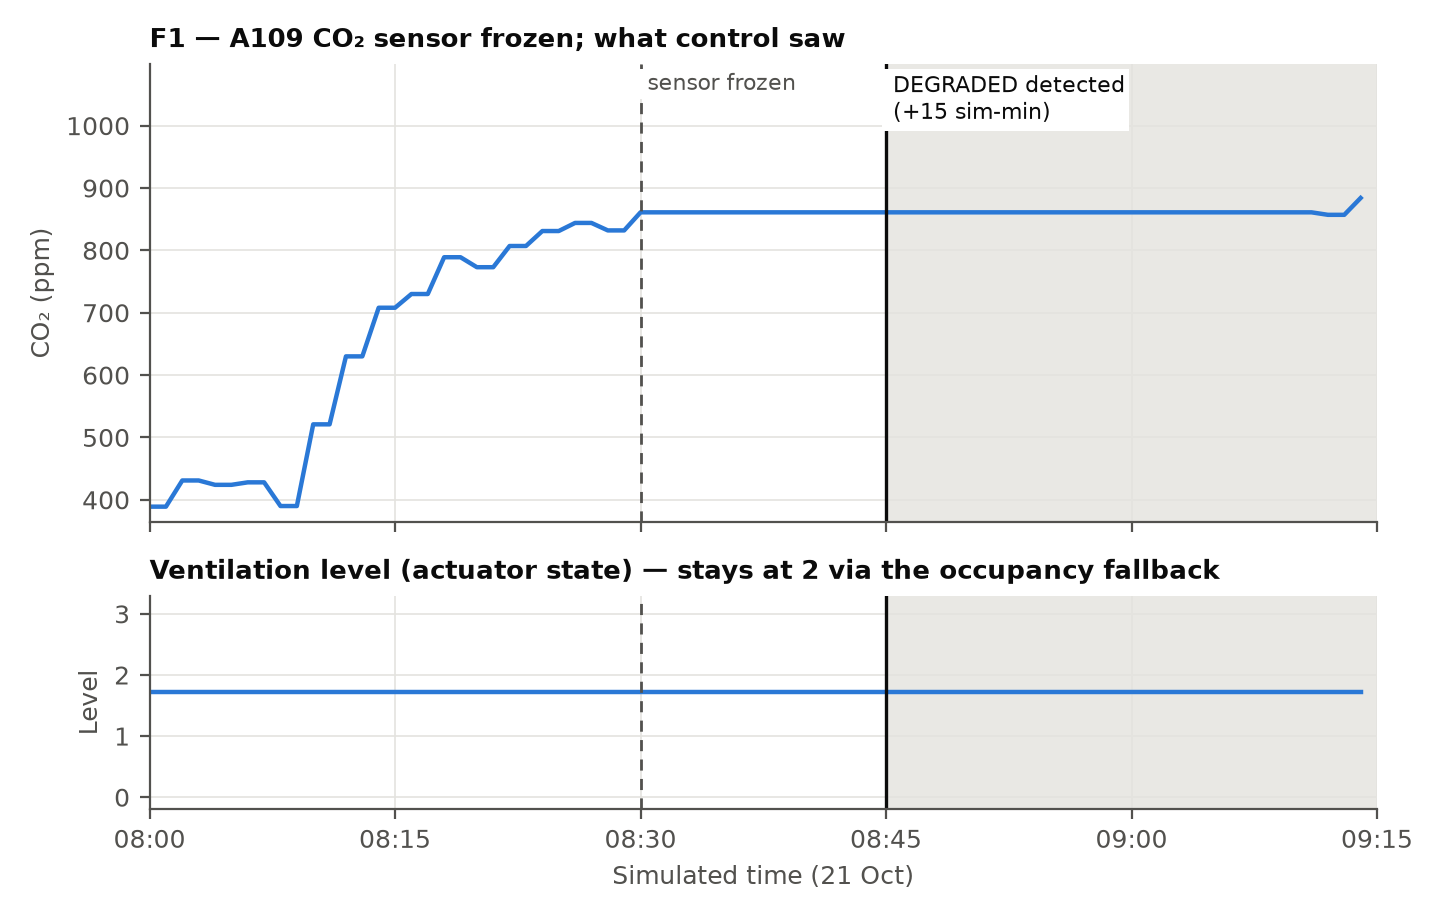
\includegraphics[width=0.85\linewidth]{f1_frozen_sensor.png}
\caption{F1: A109 CO\textsubscript{2} frozen at 08:30; control switches to DEGRADED and ventilates from the occupancy count.}\label{fig:f1}
\end{figure}

\textbf{F3a -- controller restart.} Control was stopped at wall UTC 10:18:05 and restarted at 10:18:36. The first recorded decision arrived at 10:18:42: six seconds after restart and 37 seconds after stopping. A109's actuator held level 3 during the outage. This shows prompt recovery of decisions in this case, but not that every device received correct commands.

\textbf{F3b -- actuator restart.} At clock factor 60 the retained command was still younger than 120 s and was accepted, so the test was repeated at real-time factor 1. There, the restarted actuator rejected the 154-second-old retained command. The A117 actuator stayed at level 0 while seven controller decisions continued to request level 2 without resending the unchanged target. This confirms the restart defect and fails the general NFR-02 recovery claim. The submitted version does not fix this defect; Section~\ref{sec:risks} describes the mitigation.

\textbf{F6 -- invalid commands.} Three commands were rejected and logged: foreign issuer, target 99 outside the allowed range, and a timestamp 11,888 seconds old. These cases support SAF-01 validation. A fresh command that simply claims to come from control would still be accepted.

Evidence: \protect\path{docs/results/faults.txt}.

\section{Evaluation and results}
\label{sec:results}
\paragraph{Evidence and comparison method.}
Final-configuration runs R6, R7 and R8 use simulated 21 October 2026, 07:30--18:00, factor 60 and the same occupancy seed. Control and physics were restarted and the clock reset before each variant; energy counters therefore start at zero. Observed sensors, sampled every two sim-min, were resampled per simulated minute with last-value hold. Occupied means observed occupancy greater than zero. Energy was captured from the final physics counters. The fixed-schedule baseline R9 was run under the same conditions and evaluated with the same script.

\noindent\begin{tabularx}{\linewidth}{Xrrrr}\toprule Metric & R6 reactive & R7 persistence & R8 timetable & R9 fixed schedule\\\midrule
Lecture occupied sim-min & 473 & 475 & 465 & 476\\
Lecture occupied CO\textsubscript{2} $>1000$ sim-min & 122 & 2 & 0 & 0\\
Lecture peak CO\textsubscript{2} (ppm) & 1276 & 1002 & 920 & 917\\
Lecture ventilation target changes & 36 & 17 & 10 & 2\\
Lecture occupied comfort (\%) & 70.2 & 68.8 & 84.7 & 96.4\\
All-room radiator + AHU (kWh) & 259.5 & 280.7 & 282.6 & 445.8\\\bottomrule\end{tabularx}


Both planner variants exceed FR-04's 50\% reduction criterion for the two lecture rooms: persistence reduces the exceedance minutes by about 98\%, timetable by 100\%. Timetable also improves lecture comfort to 84.7\%, still below FR-02's 90\%. Relative to reactive-only, all-room heat energy rises by about 8.2\% with persistence and 8.9\% with timetable. Figure~\ref{fig:planner} shows that the timetable variant keeps A117 below 1000 ppm across its three lectures and persistence nearly does (2 sim-min, peak 1002 ppm), while reactive control alone repeatedly overshoots; Figure~\ref{fig:s1} shows a full R8 day in A109.

\begin{figure}[H]\centering
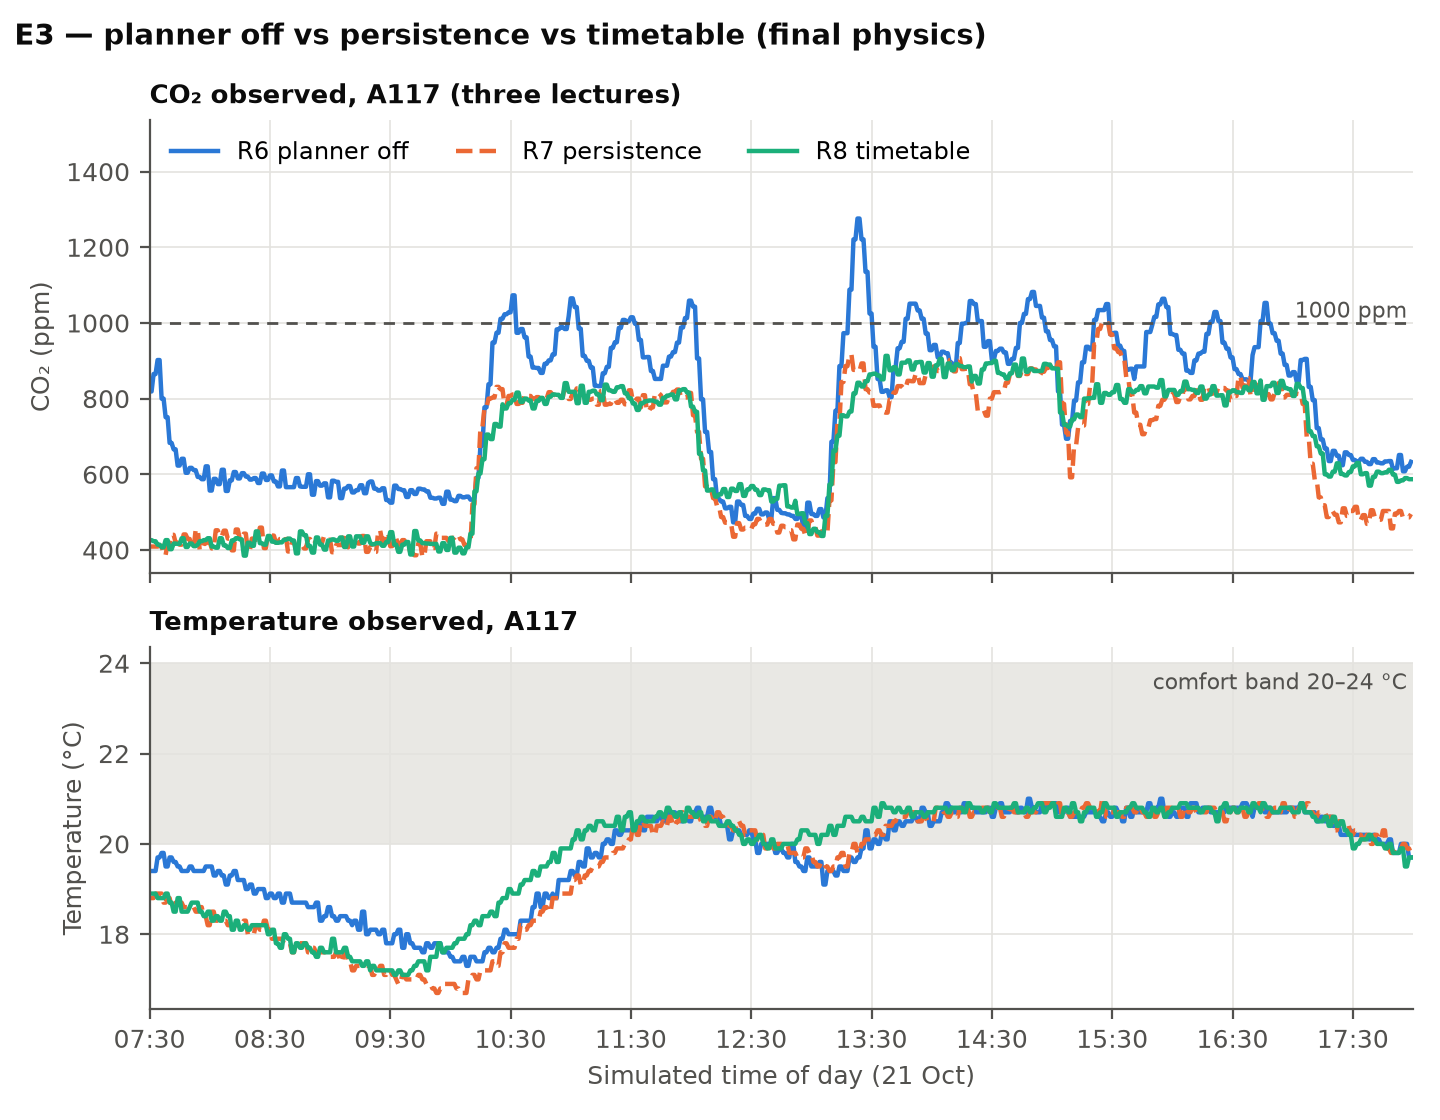
\includegraphics[width=0.9\linewidth]{e3_planner_A117.png}
\caption{A117, runs R6--R8: observed CO\textsubscript{2} and temperature with reactive control only (R6) and the two planner variants (R7, R8).}\label{fig:planner}
\end{figure}
\begin{figure}[H]\centering
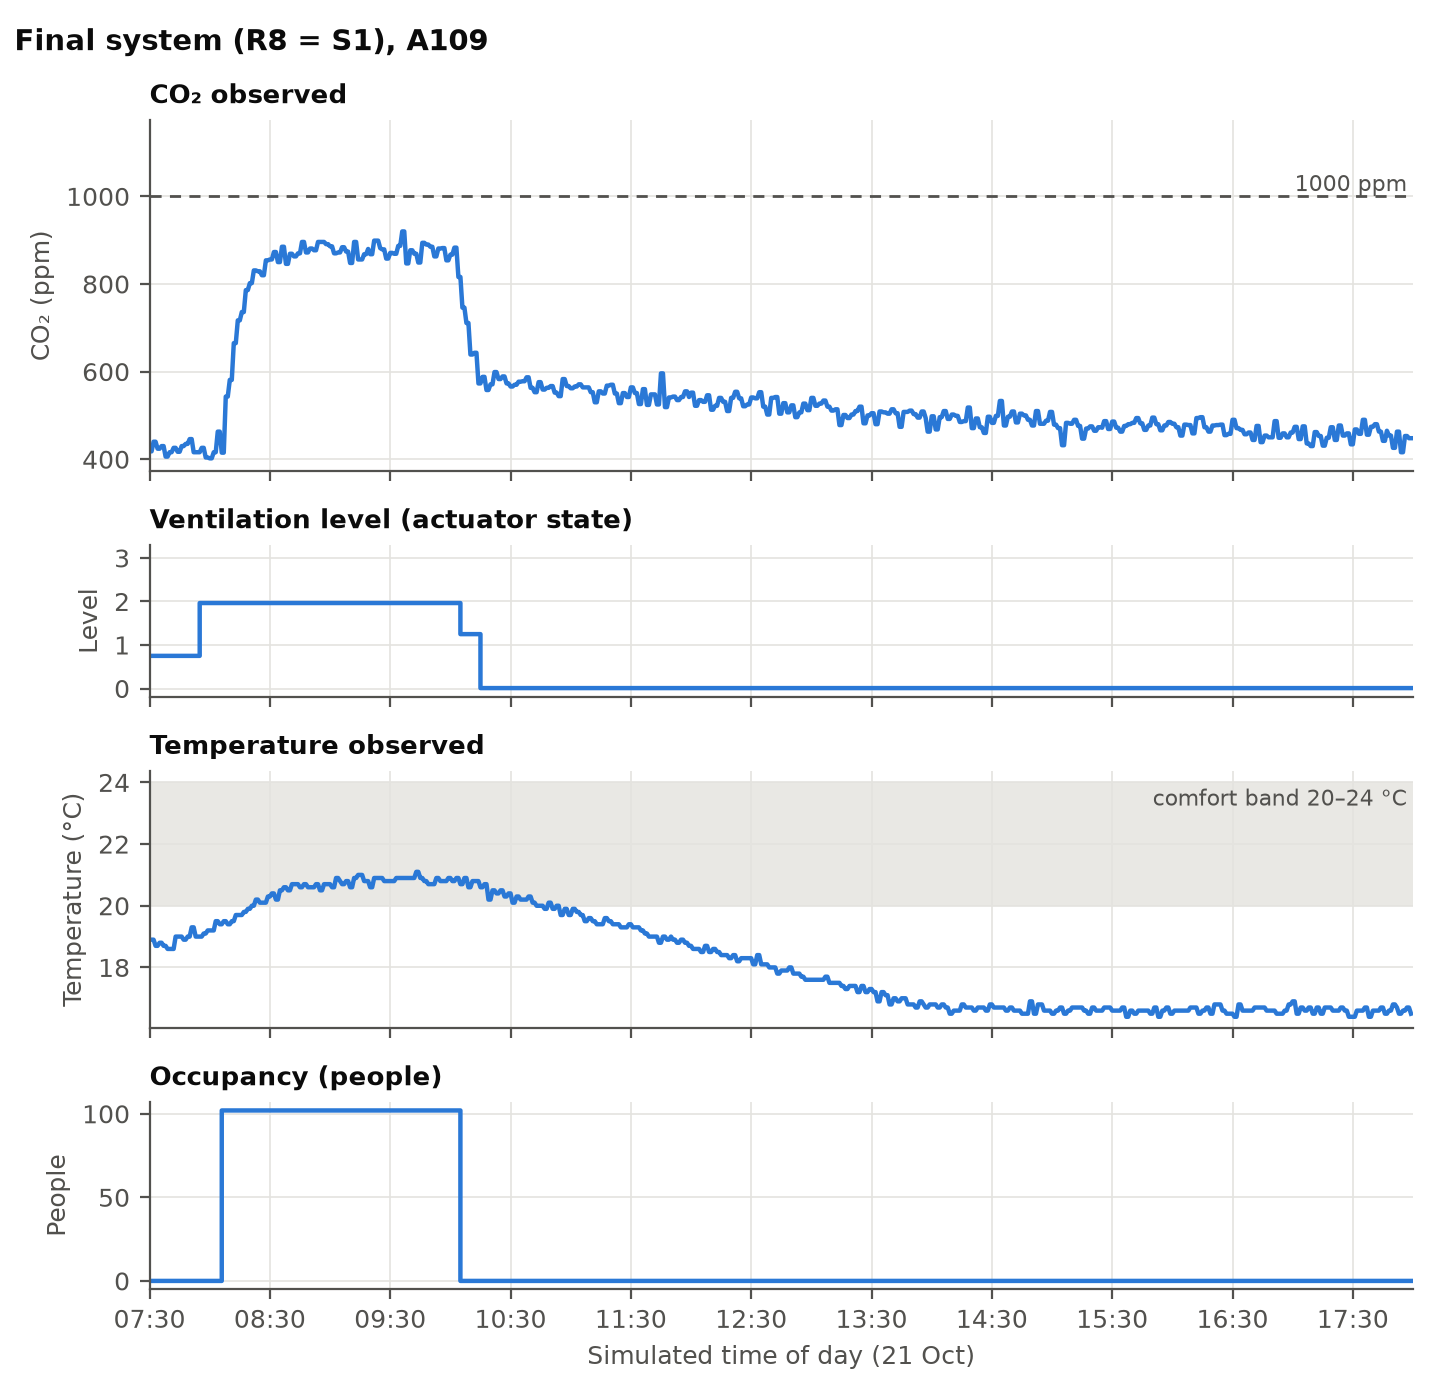
\includegraphics[width=0.8\linewidth]{s1_A109.png}
\caption{A109, run R8 (timetable): observed CO\textsubscript{2}, ventilation, temperature and occupancy over the simulated weekday.}\label{fig:s1}
\end{figure}

\paragraph{Fixed-schedule baseline (E1, NFR-04).}
R9 repeats the same simulated day with the controller replaced by a timer (\texttt{CONTROL\_MODE=fixed-schedule}): ventilation level 2 and 21 $^\circ$C from 07:30 to 17:00, level 0 and 17 $^\circ$C otherwise, without sensors or plans; the planner was stopped. Its occupied lecture minutes (476) match R6--R8 (465--475), so the conditions are comparable. The baseline used 445.8 kWh, 58\% more than R8 (282.6 kWh); the final system therefore needs 37\% less energy, and NFR-04 is met in the model. Radiators account for 104 kWh of the difference, mainly in rooms that stay heated while empty (A109 after its only lecture: +56 kWh), and AHU supply-air heating for 59 kWh, because every room is ventilated at level 2 for 9.5 simulated hours. The baseline was not worse for air quality: it also had zero lecture-room exceedances (peak 917 ppm), contrary to the prediction we recorded before the run. This indicates that R6's exceedances come from the reactive rules (a lecture starts at level 0, ventilation rises only after CO\textsubscript{2} does, and the threshold cycle described below), not from insufficient level-2 capacity; the timer is already at level 2 when students arrive, which is the effect the planner reproduces. Heating from 07:30 also gave the timer 96.4\% lecture comfort, which would meet FR-02. In the fika room it had fewer exceedance minutes (6 against 28) but a higher peak (1380 ppm), as it has no safety override. Against a conventional schedule, the autonomous system's benefit is therefore energy, paid for with lower comfort; timetable-driven preheating is the most direct improvement. One run per variant and our own choice of schedule (level 2, 07:30--17:00) make the 37\% specific to this scenario.

\paragraph{Whole-building limits.}\mbox{}\par
\noindent\begin{tabularx}{\linewidth}{lrrrX}\toprule R8 room & Exceed sim-min & Peak ppm & Comfort (\%) & Heat + AHU (kWh)\\\midrule
A109 & 0 & 920 & 87.4 & 75.2\\
A117 & 0 & 913 & 83.8 & 125.0\\
A110 & 28 & 1192 & 24.8 & 65.7\\
A323 & 0 & 468 & N/A & 6.6\\
A113C & 0 & 829 & 79.6 & 10.1\\\bottomrule\end{tabularx}
A323 had no occupied minutes, so it provides no occupied-comfort evidence. The fika room has neither booking-based anticipation nor adequate comfort in this run. Zero lecture exceedances support the air-quality outcome for those rooms and that scenario; 28 total fika exceedance minutes do not reveal whether any individual episode exceeded FR-01's ten-minute recovery deadline. A building-wide acceptance claim would require episode-level analysis and more scenarios.

\paragraph{Forecast quality and deployment decision.}
The recorded fit used 23,755 training samples from simulated 2--19 October and 1,105 held-out samples on 20 October. MAE is in persons:
\noindent\begin{tabularx}{\linewidth}{Xrrrrrr}\toprule Horizon (sim-min) & 5 & 10 & 15 & 20 & 25 & 30\\\midrule
Linear-model MAE & 2.17 & 3.97 & 5.48 & 6.90 & 8.09 & 9.21\\
Persistence MAE & 1.29 & 2.36 & 3.19 & 3.99 & 4.65 & 5.34\\\bottomrule\end{tabularx}
The linear model is worse at every horizon and was not deployed. Timetable forecasting introduces useful advance information that persistence lacks, but the simulator's complete registered attendance makes this a favourable scenario that says little about forecast accuracy in a real building.

\paragraph{Uncertainty.}
Earlier runs R1--R5 are excluded: they used the older thermal model, which gave zero comfort, and R2/R3 also used a faulty history query. There is one run per final variant. Sensor noise, clock resets and differing recorded occupied durations limit causal precision; no confidence interval is justified. Reactive results also depend on tuning: level 2 can settle below the 900-ppm step-down point, after which level 1 allows concentration to rise again. Part of the planner benefit therefore compensates for a threshold cycle.

\paragraph{Additional temperature metric.}
Most remaining comfort misses are slightly cool (18--20 $^\circ$C) rather than unsafe: within the wider 18--24 $^\circ$C range of Swedish public-health guidance (\href{https://www.folkhalsomyndigheten.se/contentassets/1c28701a4c8f49cabce85e3bb65695dc/hslf-fs-2024-10.pdf}{Folkh\"alsomyndigheten, HSLF-FS 2024:10}), R8 reaches 99.3\% of occupied lecture time (R6: 95.6\%, R7: 93.3\%) and 87.6\% in the fika room.

\paragraph{Shared-model optimism.}
The planner rollout calls the simulation's own physics step with the same parameters and outdoor-temperature formula. Consequently the evaluation has no model--plant mismatch. Exact occupancy counts and complete registered attendance also favour forecasting and occupancy-based fallback. The results are therefore optimistic simulator evidence, not real-building performance.

\section{Dashboard}
BuildSim provides the live spatial view. Viewer consumes observations, decisions and service health, then replaces the full room-layer and alert collections through REST. A single writer avoids two project services overwriting each other's layers. Room layers show the observed CO\textsubscript{2}, temperature and occupancy; alerts list rooms that are not in NORMAL mode, with the controller's reason, and services that report a problem.

Grafana reads pipeline SQL queries through the Infinity datasource and adds historical context to the 3D view; it does not control equipment. A dashboard that remains reachable can still display stale data, so timestamps and degraded status matter. Figure~\ref{fig:grafana-dashboard} shows the Grafana dashboard for A109: observed CO\textsubscript{2}, temperature, ventilation level with occupancy, and the latest decisions with their reasons.


\begin{figure}[H]
    \centering
    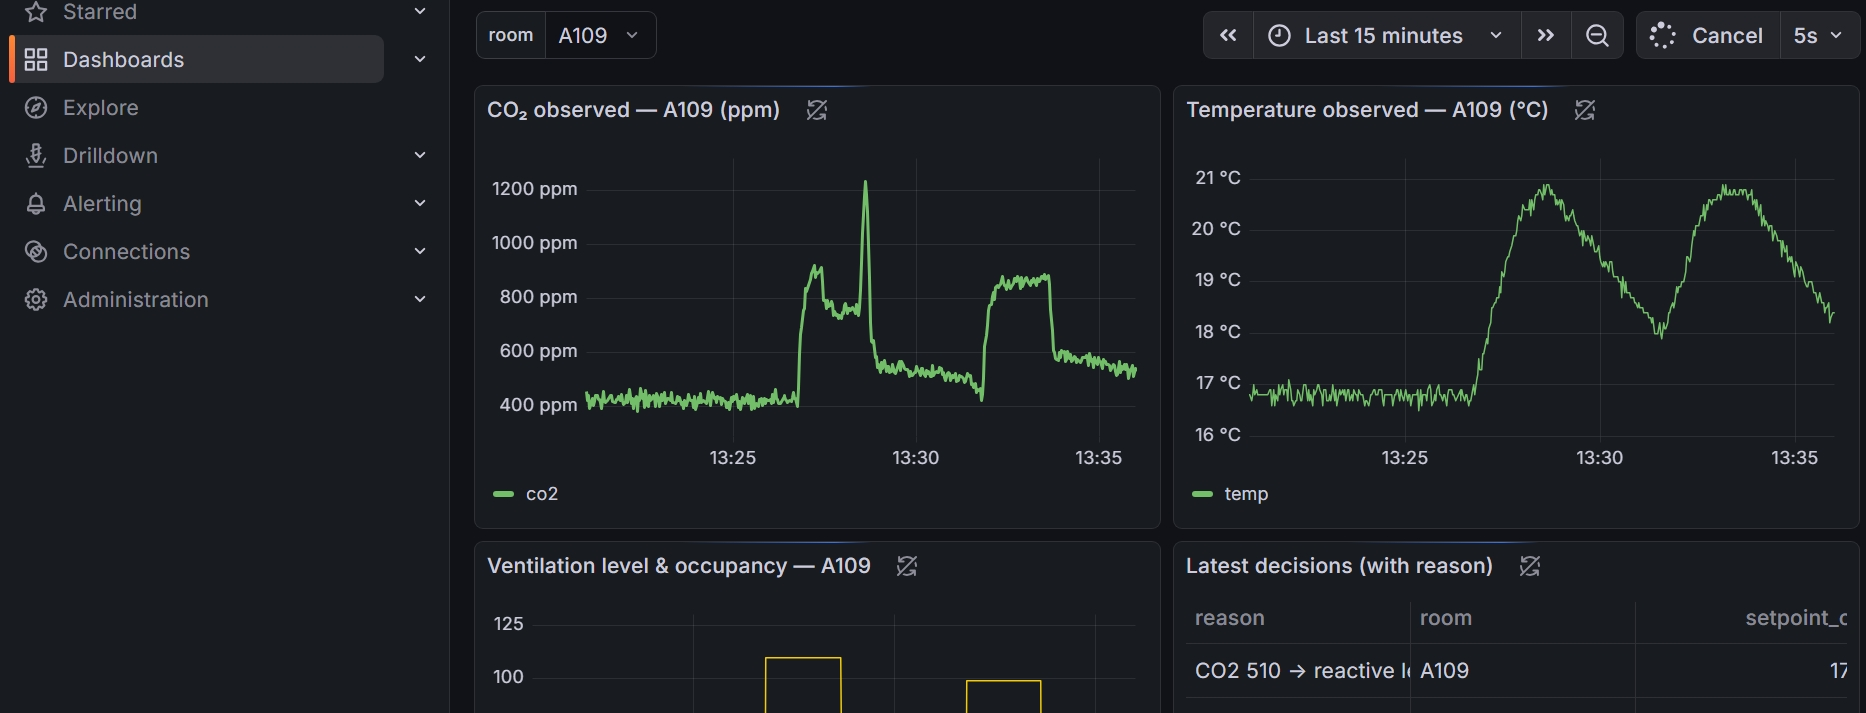
\includegraphics[width=\linewidth]{grafana_pic.jpeg}
    \caption{Grafana dashboard for A109 (live view, last 15 minutes).}
    \label{fig:grafana-dashboard}
\end{figure}

\section{Risks and critical reflection}\label{sec:risks}
\paragraph{Modelling limits.}
Perfect mixing, ideal occupancy counts, fixed parameters and synthetic weather simplify reasoning but limit transfer to a real building. Inter-room air exchange, solar gains, humidity, fan electricity and active cooling are absent. Heat-recovery efficiency and AHU capacity are assumptions. Proportional heating may settle below setpoint, and because rooms start at 19 $^\circ$C and are set back when empty, preheating needs enough lead time. Modelled kWh is only meaningful for comparing variants.

{\small\begin{longtable}{>{\raggedright\arraybackslash}p{36mm}>{\raggedright\arraybackslash}p{52mm}>{\raggedright\arraybackslash}p{56mm}}\toprule Risk & Consequence & Next mitigation\\\midrule\endhead
Frozen, drifting or stale observations & Late fallback or wrong demand & Detect frozen values by elapsed time; add plausibility and drift checks.\\
Retained command and no acknowledgement & Restarted actuator keeps a stale target & Resend targets periodically and compare reported states with targets.\\
Timetable attendance assumption & Unnecessary heating or missed unscheduled demand & Attendance uncertainty and observed-occupancy correction; improve fika handling.\\
Shared broker, BuildSim and host & Correlated room failures & Measure outage behaviour; process isolation gives no host redundancy.\\
Cross-run history and duplicates & Wrong forecasts or biased metrics & Run and event identifiers; queries partitioned by run.\\
Growing file scans and storage & Query latency and memory growth & Retention bounds and incremental partitioned compaction.\\
Uncalibrated heat and energy model & Misleading comfort or energy comparison & Correct the weather phase, calibrate parameters and store energy counters persistently.\\
Unauthenticated APIs and topics & Spoofed commands, fault injection, unrestricted queries, access to the physics truth API & Authentication, ACLs, TLS and narrower query access before broader use.\\\bottomrule\end{longtable}}

\paragraph{Next steps.}
With more time, we would first address the quality and recovery gaps: frozen detection by elapsed time, plausibility and timestamp checks on inputs and commands, periodic command refresh and a check that reported actuator states match their targets. We would also introduce run and event identifiers to separate replayed runs and remove duplicates, and store radiator and AHU energy persistently instead of only in the physics process.

We would then improve comfort and decision quality: extend timetable-driven preheating, use observed temperature in heat decisions, retune reactive hysteresis as a simpler comparator, and improve handling of unscheduled fika demand. The weather phase would be corrected and the thermal and flow parameters calibrated. Attendance-aware forecasts would be compared against persistence on independent dates and seeds before any learned model is deployed.

Finally, we would strengthen the evidence: repeat all four variants, including the fixed-schedule baseline, over several days and seeds, and add episode-level CO\textsubscript{2} recovery, setback timing, fault and restart recovery, loss checks and scaling to a breaking point, preserving configuration, seed, model version and run windows with every result. The recorded evidence supports a conditional lecture-room improvement; comfort, unscheduled rooms and operational guarantees are where the system falls short.

\section*{Contribution statement}\addcontentsline{toc}{section}{Contribution statement}
\noindent{\small\begin{tabularx}{\linewidth}{>{\raggedright\arraybackslash}p{25mm}>{\raggedright\arraybackslash}X>{\raggedright\arraybackslash}X>{\raggedright\arraybackslash}X}\toprule
Area & Both & Tobias Hanke & Evangelos Vasilaras\\\midrule
Architecture & Use case and proposal; architecture decisions (service split, MQTT, storage, Python) & -- & C4/D2 diagrams and architecture documentation\\
Implementation & System setup and bring-up of all containers; Grafana dashboard & Physics and ventilation model changes; timetable planner; history replay fix & --\\
Testing & Unit tests, end-to-end test, stability run & Fault injection F1, F3, F6 & --\\
Evaluation & Comparison runs R1--R9; forecast evaluation E5 & -- & --\\
Report & Writing and revision & Result figures; final revision & First complete LaTeX draft; diagram redrawing\\\bottomrule
\end{tabularx}}

\smallskip\noindent We used AI assistance (Claude) to write most of the code and to draft the report. Both members defined the use case and the architecture decisions, ran and checked the experiments, and reviewed code and text throughout, finding and correcting many errors.

\section*{References}\addcontentsline{toc}{section}{References}
{\small\begin{itemize}
\item Folkh\"alsomyndigheten (Public Health Agency of Sweden): HSLF-FS 2024:10, general advice on indoor temperature. \url{https://www.folkhalsomyndigheten.se/contentassets/1c28701a4c8f49cabce85e3bb65695dc/hslf-fs-2024-10.pdf}
\item Folkh\"alsomyndigheten: FoHMFS 2014:18, Folkh\"alsomyndighetens allm\"anna r\aa d om ventilation. \url{https://www.fohm.se/contentassets/641784832543443ea4eebe9b300c244e/fohmfs-2014-18.pdf}
\item NOAA Global Monitoring Laboratory: Trends in atmospheric carbon dioxide, global monthly means (accessed 12 October 2026). \url{https://gml.noaa.gov/ccgg/trends/global.html}
\end{itemize}}

\end{document}
